\subsection{AzuDICI}
\label{sec:azudici}

We already know that the problem with cache-misses is tightly related
to the way in which BCP is implemented \cite{paper cache misses sat} and,
therefore, with the way in which clauses and watches are programmed.
Since \pling keeps a separate clause database for each thread, it is 
possible that sharing data could improve cache performance, because
we would have a smaller amount of total data to propagate with.
Based on other parallel SAT-solvers that share their clause database, 
mainly {\tt SArTagnan} and {\tt MiraXT}, we decided to implement AzuDICI, 
a basic CDCL SAT-solver with the purpose of improving the BCP performance
in portfolio-approach SAT-solvers.
Three versions of AzuDICI were implemented, one in which each thread keeps
a separated database clause; another in which, as in MiraXT, shares all
clauses physically; and an hybrid third one which only shares binary
implication lists.

\subsubsection{AzuDICI general structure}

AzuDICI\footnote{You can find the latest implementation of AzuDICI at
  \url{https://github.com/leoferres/AzuDICI}} is a standard CDCL
solver based on \pling, {\tt barcelogic} and {\tt miraXT}.
In particular, AzuDICI implements binary implication lists for the
propagation with binary clauses, and the two-watched literals scheme
for unit propagation \cite{} with clauses of more than two
literals. AzuDICI also implements the 1-UIP algorithm for conflict
analysis \ref{}, the lemma simplification algorithm used in {\tt
  PicoSAT}, Luby restarts \cite{}, a policy for lemma cleaning that
keeps only binary and ternary lemmas, and more than four-literal
lemmas that have participated in a conflict since the last
cleanup. Finally, AzuDICI also incorporates the EVSIDS heuristic for
branching literal decisions \cite{}.

\subsubsection{Shared-none}

This version works as plingeling, it doesn't share any clause physically. 
Each thread keeps its own independent database of clauses and propagates 
with it. Note that the fact that we are not sharing data physically 
doesn't mean threads can't share information. They could very well, for 
example, share unit clauses through message passing between threads, just 
as \pling does. We are interested in measuring the impact in cache 
performance of sharing data physically, and not the benefits of sharing 
information by it self.

\subsubsection{Shared-bins}

\begin{figure}[tp]
  \centering
  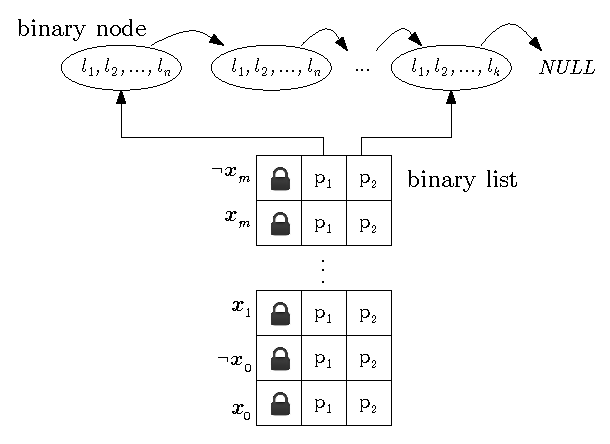
\includegraphics[scale=1.0]{implication_list}
  \caption{Binary clause database}
  \label{fig:shared bins}
\end{figure}

The Shared-bins version shares the binary implication lists. All threads 
have access to the same physical data, they all can modify and read this 
structure. Figure \ref{fig:shared bins} is a schematization of our 
binary implication lists structure. We have an array of \textit{binary 
lists}, one for each literal. A binary list is basically two pointers, 
one to a first \textit{binary node} and another to the last binary node 
associated with that list. A 
binary node is an array of literals that also has a pointer to another 
binary node. The amount of literals a binary node can hold will depend 
on the size of the cache line we are working with; it will have as many 
literals as a cache line can hold. The literals implied by the literal 
associated to a binary list will be the ones in the binary node 
referenced by that binary list pointer and the subsequently referenced 
binary nodes. 

When a thread wants to add the clause $\{l_i,l_j\}$, it must look for 
the binary list associated with $\neg l_i$ and go to the last node linked 
to that binary list. If there is enough space in that node to add 
another literal, then it adds $l_j$. If the node is full, then it must 
create a new node with the $l_j$ literal, insert it at the end of the 
linked list of nodes, 
updating the binary list last node pointer. It does the same for the 
binary list of $\neg l_j$.

To ensure consistency of 
data when multiple threads are inserting, each binary list has a lock. 
If a thread is inserting a new implicated literal, it first locks the 
binary list where it's inserting and then proceeds to insert. If by 
chance another thread wants to insert in the same binary list, it must 
wait till the lock is freed. Since adding binary clauses is not a 
frequent event, and even less frequent the event that it would happen 
in the same binary list, the contention that these locks generate is 
unnoticeable in our experimental results.


\subsubsection{Shared-all}

\begin{figure}[tp]
  \centering
  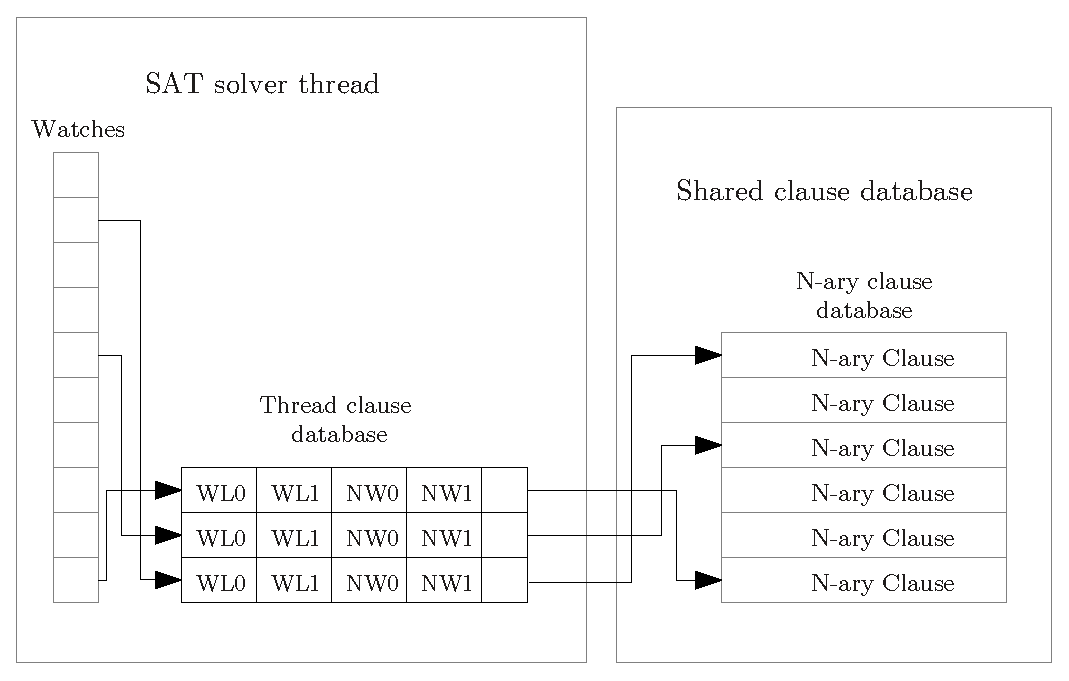
\includegraphics[scale=0.6]{AzuDICI_design}
  \caption{The thread clause database and n-ary clause database}
  \label{fig:azu design}
\end{figure}

In the shared-bins solver we had no need to modify the usual two 
watched literal scheme used in propagation. This is not
the case for this version that shares n-ary clauses physically. 
The two watched literal scheme requires to make changes to the 
clause in order to identify 
the literals being watched at one given instant (for example, place
both literals first in the clause). Since many threads will be
accessing the same clauses, these changes to the clause are not
feasible to share n-ary clauses. Instead, we have used a similar 
approach as used in
{\tt miraXT}, where each thread keeps track of the literals being
watched in each clause. Figure \ref{fig:azu design} is a
schematization of how each thread worker relates with the n-ary
clause database. Each SAT solver thread has a vector of pointers
to thread clauses called \textit{watches}, and each literal present
in the SAT problem has a position associated in this watches vector.
A thread clause has two watched literals (WL0 and WL1), two
pointers to another thread clause (NW0 and NW1) and a pointer to
an actual n-ary clause in the n-ary clause database. W0 and W1 keep
track of the literals being watched by the thread for a given n-ary
clause. NW0 and NW1 point to the next thread clauses that are also 
watching WL0 and WL1 respectively. The n-clause also has a flag for 
each worker thread to identify which ones are using that clause 
for propagation.

To insert a new n-ary clause, we first make sure that the clause 
doesn't exist in the database [vale la pena explicar como lo hace?]. If it 
doesn't exist, we create the n-clause, set the current thread 
flag to true and add it to the database. 
On the other hand, if it does exist, we just toggle the 
corresponding thread flag of the n-clause to true. The inserting 
procedure is locked so that two different threads can't insert
at the same time. In our experiments we haven't noticed any 
considerable overhead caused by this lock.

%%% Local Variables: 
%%% mode: latex
%%% TeX-master: "sat"
%%% End: 
